\documentclass[12pt]{article}

% Popup for cipher
\usepackage{pdfcomment}
% Draw Caesar cipher / LFSR
\usepackage{tikz}
\usetikzlibrary{matrix,positioning,calc,fit}
\tikzset{circ/.style={draw,circle,node distance=2mm,inner sep=0.1pt},topath/.style={to path={|-(\tikztotarget)}}}

\usepackage{ifthen}
% Be able to get substrings
\usepackage{xstring}

% Caesar cipher drawing
\newcounter{index}
%command to increase a counter by 1 modulo 26
\newcommand{\increase}[1]{\ifthenelse{\arabic{#1}<26}{\addtocounter{#1}{1}}{\setcounter{#1}{1}}}
\newcommand{\pOneCipher}{CBDGFAIELKHJMSNQOPURVTYWXZ}
\newcommand{\pOneKey}{ETANORSICLHDUPMGWFVYKBXJQZ}

% Standard
\usepackage[top=0.8in,bottom=0.8in]{geometry}
\usepackage{amsmath,bm}
\usepackage{amssymb}
\usepackage{enumitem}
\usepackage{graphicx}
\usepackage{tcolorbox}
\usepackage{array,multirow}
\usepackage{mathtools}
\DeclarePairedDelimiter{\ceil}{\lceil}{\rceil}
\DeclarePairedDelimiter\floor{\lfloor}{\rfloor}
% Enables font change size in verbatim blocks
\makeatletter
\newcommand{\verbatimfont}[1]{\renewcommand{\verbatim@font}{\ttfamily#1}}
\makeatother
\usepackage{hyperref}
\hypersetup{
    colorlinks=true,
    linkcolor=blue,
    filecolor=magenta,      
    urlcolor=cyan,
}
 
\urlstyle{same}


% Format for answering questions
\newenvironment{answer}
{ \begin{tcolorbox}[halign=left]
    }
    {  
  \end{tcolorbox}
}

\begin{document}

\title{CS 4801: Assignment 2}
\author{Adam Camilli (aocamilli@wpi.edu)}
\date{\today}
\maketitle

\begin{enumerate}

\item \textbf{DES}
\\

% input: 1100 1000 1010 0110 1011 0011 0000 1111
% key: 10001011 01000000 01011011 00101110 01110111 10001011
    \centerline{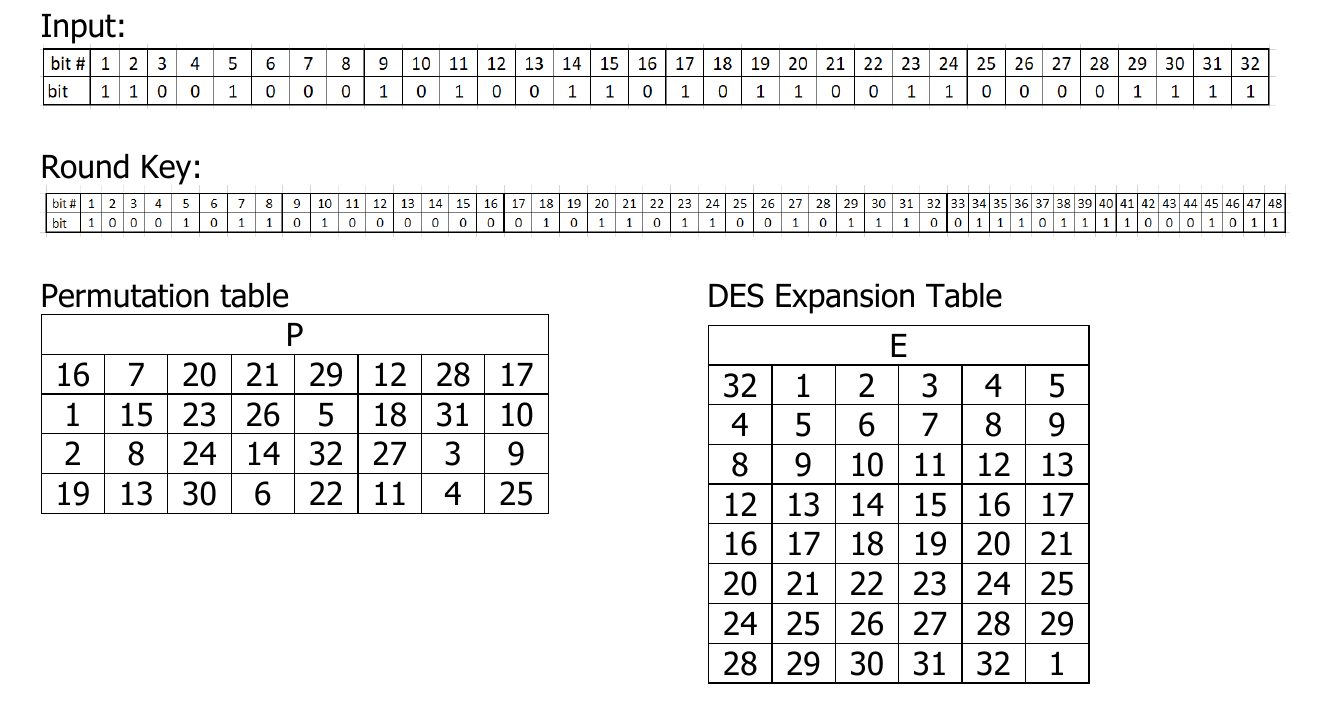
\includegraphics[width=1.3\textwidth]{pictures/DES}}
    \newpage
    \begin{enumerate}
    \item Extend the input to 48 bits using DES expansion function
      \begin{answer}
        Using expansion table, we populate a new 48-bit string:
        \begin{center}
          \begin{tabular}{|c|c|c|c|c|c|}
          \hline
          1 (32) & 1 (1) & 1 (2) & 0 (3) & 0 (4) & 1 (5) \\ 
          \hline
          0 (4) & 1 (5) & 0 (6) & 0 (7) & 0 (8) & 1 (9) \\ 
          \hline
          0 (8) & 1 (9) & 0 (10) & 1 (11) & 0 (12) & 1 (13) \\ 
          \hline
          0 (12) & 0 (13) & 1 (14) & 1 (15) & 0 (16) & 1 (17) \\ 
          \hline
          0 (16) & 1 (17) & 0 (18) & 1 (19) & 1 (20) & 0 (21) \\ 
          \hline
          1 (20) & 0 (21) & 0 (22) & 1 (23) & 1 (24) & 0 (25) \\ 
          \hline
          1 (24) & 0 (25) & 0 (26) & 0 (27) & 0 (28) & 1 (29) \\ 
          \hline
          0 (28) & 1 (29) & 1 (30) & 1 (31) & 1 (32) & 1 (1) \\ 
          \hline
        \end{tabular}
      \end{center}
      This extends input to
      \[ 111001010001010101001101010110100110100001011111 \]
      \end{answer}
    \item Add (XOR) the given round key to the expanded input bits.
      \begin{answer}
        $111001010001010101001101010110100110100001011111$ (Expanded input)\\
        \hspace{5.8cm} $\oplus$ \\
        $100010110100000001011011001011100111011110001011$ (Key) \\
        --------------------------------------------- \\
        $011011 100101 010100 010110 011101 000001 111111 010100$ \\
      \end{answer}
    \item Using 8 DES S-boxes, find the 32-bit output of substitution step. DES S-boxes are
      presented in the DES paper, appendix 1 (pages 17-18).
      \begin{answer}
        Note $S$-rows and columns start at zero.
        \begin{center}
          \begin{tabular}{|c|c|c|c|c|}
            \hline
            \textbf{Box} & \textbf{Input} & \textbf{Row} & \textbf{Col} & \textbf{Sub} \\
            \hline
            $S_1$ & 011011 & 01 (R2) & 1101 (C14) & 5 (0101) \\
            \hline
            $S_2$ & 100101 & 11 (R4) & 0010 (C3) & 8 (1000)\\
            \hline
            $S_3$ & 010100 & 00 (R1) & 1010 (C11) & 6 (0110)\\
            \hline
            $S_4$ & 010110 & 00 (R1) & 1011 (C12) & 12 (1100) \\
            \hline
            $S_5$ & 011101 & 01 (R2) & 1110 (C15) & 3 (0011)\\
            \hline
            $S_6$ & 000001 & 01 (R2) & 0000 (C1) & 0 (0000) \\
            \hline
            $S_7$ & 111111 & 11 (R4) & 1111 (C16) & 13 (1101) \\
            \hline
            $S_8$ & 010100 & 00 (R1) & 1010 (C11) & 6 (0110) \\
            \hline
        \end{tabular}
      \end{center}
      This reduces output to 
      \[ 0101 1000 0110 1100 
        0011 0000 1101 0110 \]
      \end{answer}
\newpage
    \item Permute the S-box output using the given permutation table.
      \begin{answer}
        \begin{center}
          \begin{tabular}{|c|c|c|c|c|c|c|c|}
            \hline
            0 (16) & 0 (7) & 1 (20) & 0 (21) & 0 (29) & 0 (12) & 1 (28) & 0 (17) \\
            \hline
            0 (1) & 0 (15) & 0 (23) & 1 (26) & 1 (5) & 0 (18) & 1 (31) & 1 (10) \\
            \hline
            1 (2) & 0 (8) & 0 (24) & 1 (14) & 0 (32) & 0 (27) & 0 (3) & 0 (9) \\
            \hline
            1 (19) & 1 (13) & 1 (30) & 0 (6) & 0 (22) & 1 (11) & 1 (4) & 1 (25) \\
            \hline            
          \end{tabular}
        \end{center}
        \[ 0010 0010 0001 1011 1001 0000 1110 0111 \]
      \end{answer}
  
    \end{enumerate}

\item \textbf{AES}
\\~\\
  \centerline{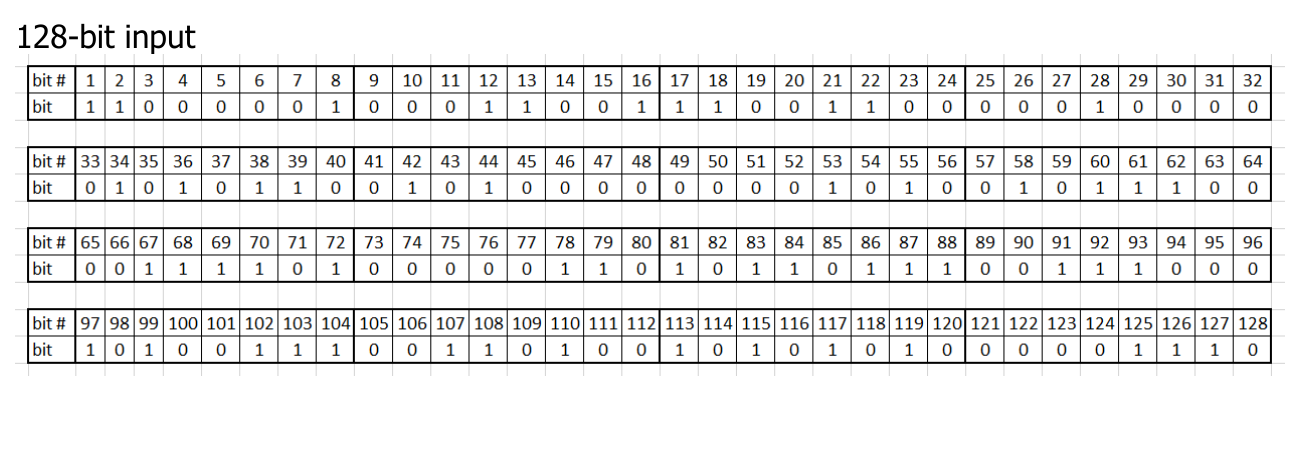
\includegraphics[width=1.1\textwidth]{pictures/AES_1}}
\\
\centerline{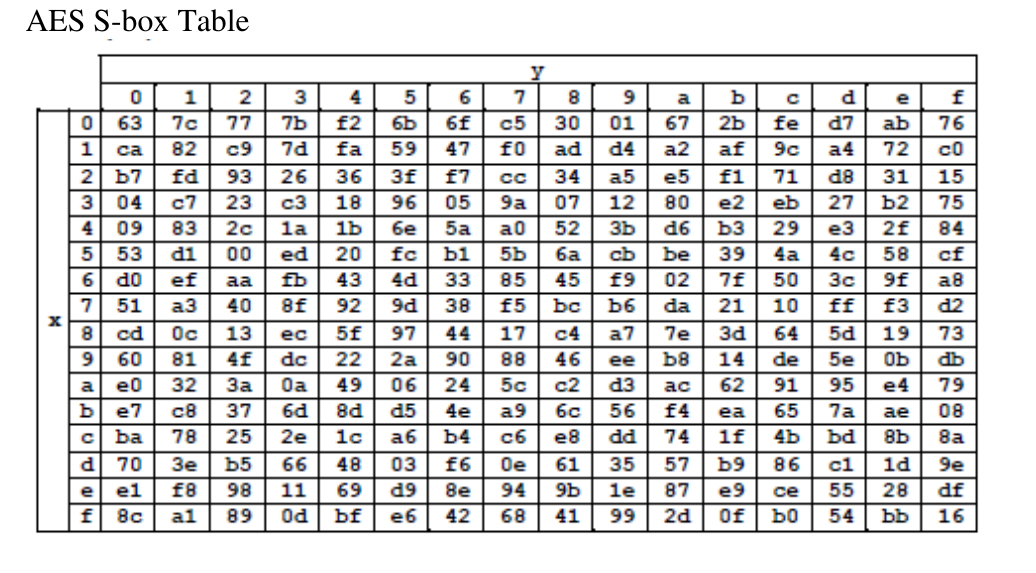
\includegraphics[width=1.1\textwidth]{pictures/AES_2}}
\newpage
% input: 
11000001 00011001 11001100 00010000
01010110 01010000 00001010 01011100
00111101 00000110 10110111 00111000
10100111 00110100 10101010 00001110


  \begin{enumerate}
    \item Write the given input to Hexadecimal form.
      \begin{answer}
        $11000001\text{ }00011001 \ldots 00001110_{2} = $ \\
        0C 11 9C C1 01 59 42 97 3D 06 B7 32 29 CD 2A 8$\text{E}_{16} $
      \end{answer}
    \item Write the input in a state diagram ( 4 by 4 matrix)
      \begin{answer}
        \[ 
          \begin{bmatrix}
            0C & 01 & 3D & 29 \\
            11 & 59 & 06 & CD \\
            9C & 42 & B7 & 2A \\
            C1 & 97 & 32 & 8E \\
          \end{bmatrix}
        \]
      \end{answer}
    \item Use AES S-box to substitute the given input.
      \begin{answer}
        \[ 
          \begin{bmatrix}
            0C & 01 & 3D & 29 \\
            11 & 59 & 06 & CD \\
            9C & 42 & B7 & 2A \\
            C1 & 97 & 32 & 8E \\
          \end{bmatrix}
          =
          \begin{bmatrix}
            S'_{0,C} & S'_{0,1} & S'_{3,D} & S'_{2,9} \\
            S'_{1,1} & S'_{5,9} & S'_{0,6} & S'_{C,D} \\
            S'_{9,C} & S'_{4,2} & S'_{B,7} & S'_{2,A} \\
            S'_{C,1} & S'_{9,7} & S'_{3,2} & S'_{8,E} \\
          \end{bmatrix}
          \] 
          \[ 
            =
          \begin{bmatrix}
            FE & 7C & 27 & A5 \\
            82 & CB & 6F & BD \\
            DE & 83 & A9 & E5 \\
            BA & 88 & 23 & 19 \\
          \end{bmatrix}
        \]
      \end{answer}
  \end{enumerate}
  
\item \textbf{-}
  \begin{enumerate}
  \item Find $17^{-1} \bmod 43$ using Extended Euclidean Algorithm
    \begin{answer}
      During each step $s_i$, recursively calculate  
      \[p_i = p_{i-2} - p_{i-1}q_{i-2} \bmod n \]
      $q_i$ is equal to the coefficient on the left side (bolded). Repeat until remainder is 0 and iterate right side ($p$ calcuation) one more time.
      \[\texttt{gcd(}17,43\texttt{)} = 1 \]
      \[ \therefore \text{$\exists$ integers $(p,n) \mid 17p = 43n + 1$} \]
      \begin{align*}
        &s_0: \text{  }43 = \bm{2}(17) + 9 &p_0 &= 0 \text{ (given)}\\
        &s_1: \text{  }17 = \bm{1}(9) + 8 &p_1 &= 1 \text{ (given)}\\
        &s_2: \text{  }9 = \bm{1}(8) + 1 &p_2 &= p_0 - p_1(q_0) \bmod 43 \\ 
        & & &= 0 - 1(2) \bmod 43 = 41 \\
        &s_3: \text{  }8 = \bm{8}(1) + 0 &p_3 &= p_1 - p_2(q_1) \bmod 43 \\
        & & &= 1 - 41(1) \bmod 43 = 3 \\
        & &p_4 &= p_2 - p_3(q_2) \bmod 43 \\
        & & &= 41 - 3(1) \bmod 43 = \bm{38}
      \end{align*}
      Modular inverse is \textbf{38}
    \end{answer}
    \newpage
  \item Find the inverse of $Q(x) = x^2 + 1$ in \textit{GF}($2^3$) with $P(x) = x^3 + x^2 + 1$ using Extended Euclidean Algorithm.
        \begin{answer}
          We want to find the inverse of $Q(x)$ in the field $\cfrac{GF(2^3)}{P(x)}$, which is the same as finding a polynomial $F(x)$ such that 
          \[ QF \equiv 1 (\bmod \text{ }P) \]
          or equivalently
          \[ QF + PG = 1,  G(x) \in \cfrac{GF(2^3)}{P(x)} \]
          Using the extended Euclidean algorithm, we can back-substitute from a greatest common divisor calculation (if and only if the result is 1):
          \begin{align*}
            x^3 + x^2 + 1 &= (x+1)(x^2 + 1) - x \\
            x^2 + 1 &= (-x)(-x) + 1 \\ 
          \end{align*}
          \begin{align*}
            1 &= (x^2 + 1) - (-x)(-x) \\
              &= (x^2 + 1) - (-x)((x^3 + x^2 + 1) - (x+1)(x^2 + 1)) \\
              &= Q - (-x)(F - (x+1)(Q)) \\
              &= Q - (x)(x+1)(Q) - (-x)P \\
              &= (1 - (x)(x+1))Q + (x)P \\
              &= (-x^2 -x + 1)Q + (x)P \\
              &= (x^4 - x^4 + x^3 - x^3 + x^2 - x^2 + x - x + 1) = 1
          \end{align*}
          This is verified by the final equation as well as the fact that the coefficient of $P(x)$ $G = x \in \cfrac{GF(2^3)}{P(x)}$.\\
      The inverse of $Q(x)$ is therefore $\bm{-x^2 - x + 1}$.
    \end{answer}
    \newpage
  \item Multiply $x^2+1$ by $x^2 + x + 1$ in \textit{GF}($2^3$) with $P(x) = x^3 + x^2 + 1$
    \begin{answer}
      Given that the multiplication is performed in a Galois field of form $(2^n)$, this can be performed by binary multiplication of the coefficients:
      \[ (1)x^2 + (0)x^1 + (1)x^0 \rightarrow 101 \]
      \[ (1)x^2 + (1)x^1 + (1)x^0 \rightarrow 111 \]
      \begin{align*}
        101 \cdot 111 &= 101 + 101 \cdot 10 + 10101 \cdot 10 \cdot 10 \\
                      &= 101 + 1010 + 10101 \\
                      &= \bm{11011} \\
      \end{align*}
      The result is 
      \[ \bm{1}x^4 + \bm{1}x^3 + \bm{0}x^2 + \bm{1}x^1 + \bm{1}x^0  \]
    \end{answer}
  \end{enumerate}

\end{enumerate}

\end{document}